%% Exemplo de utilizacao do estilo de formatacao normas-utf-tex (http://normas-utf-tex.sourceforge.net)
%% dúvidas acessar o site acima
%%
%%
%% Autores: (200?-2011) Hugo Vieira Neto (hvieir@utfpr.edu.br)
%%          (200?-2011) Diogo Rosa Kuiaski (diogo.kuiaski@gmail.com)
%%          (2011-2017) Marcos Talau <talau@users.sourceforge.net>
%% Colaborador:
%%          (2011) César M. Vargas Benitez <cesarvargasb@gmail.com>

%%
%% IMPORTANTE: O texto está escrito com acentuação antiga, atualmente você
%%             pode escrever acentos sem precisar de códigos para tal.
%%

\documentclass[openright]{normas-utf-tex} %openright = o capitulo comeca sempre em paginas impares
%\documentclass[oneside]{normas-utf-tex} %oneside = para dissertacoes com numero de paginas menor que 100 (apenas frente da folha) 

% force A4 paper format
\special{papersize=210mm,297mm}

\usepackage[alf,abnt-emphasize=bf,bibjustif,recuo=0cm, abnt-etal-cite=2, abnt-etal-list=99]{abntcite} %configuracao correta das referencias bibliograficas.

\usepackage[utf8]{inputenc} % pacote para acentuacao direta
\usepackage{amsmath,amsfonts,amssymb} % pacote matematico
\usepackage{graphicx} % pacote grafico
\usepackage[final]{pdfpages} % adicao da ata
\usepackage{float}

%Podem utilizar GEOMETRY{...} para realizar pequenos ajustes das margens. Onde, left=esquerda, right=direita, top=superior, bottom=inferior. P.ex.:
%\geometry{left=3.0cm,right=1.5cm,top=4cm,bottom=1cm} 

% ---------- Preambulo ----------
\instituicao{Federal University of Technology - Paraná} % nome da instituicao
\programa{Department of Electronics} % nome do programa
\area{Electronics Engineering} % [Engenharia Biomedica] ou [Informatica Industrial] ou [Telematica]

\documento{Undergraduate Thesis}
\nivel{Bacharelado} % [Mestrado] ou [Doutorado]
\titulacao{Bacharel} % [Mestre] ou [Doutor]

\titulo{{zCart: A smart cart prototype}} % titulo do trabalho em portugues
\title{\MakeUppercase{zCart: A smart cart prototype}} % titulo do trabalho em ingles

\autor{Flávio Shigueo Miamoto} % autor do trabalho
\autordois{João Pedro Zanlorensi Cardoso} % autor do trabalho
\cita{MIAMOTO, Flavio; ZANLORENSI, Joao Pedro} % sobrenome (maiusculas), nome do autor do trabalho

\palavraschave{Artificial Inteligenge, Deep Learning, Smart Devices, Internet of Things} 

\comentario{\UTFPRdocumentodata\ presented to the \UTFPRprogramadata\ of the \ABNTinstituicaodata\ as a partial requisite for obtaining the Bachelor in Electronics Engineering degree}

\orientador{André Eugênio Lazaretti, Ph.D}

\local{Curitiba} % cidade
\data{\the\year} % ano automatico

% desativa hifenizacao mantendo o texto justificado.
% thanks to Emilio C. G. Wille
\tolerance=1
\emergencystretch=\maxdimen
\hyphenpenalty=10000
\hbadness=10000
\sloppy

%---------- Inicio do Documento ----------
\begin{document}

\capa % geracao automatica da capa
\folhaderosto % geracao automatica da folha de rosto

% dedicatoria
\begin{dedicatoria}
    To all our families and their unconditional support
\end{dedicatoria}

% agradecimentos (opcional)
\begin{agradecimentos}
    We thank everyone that helped
\end{agradecimentos}

% epigrafe (opcional)
\begin{epigrafe}
 If have seen further it is by standing on the shoulders of giants.  \\
- Sir Isaac Newton
\end{epigrafe}

%abstract
\begin{abstract}
Abstract text (maximum of 500 words).
\end{abstract}

% listas (opcionais, mas recomenda-se a partir de 5 elementos)
\listadefiguras % geracao automatica da lista de figuras
\listadetabelas % geracao automatica da lista de tabelas
% \listadequadros % adivinhe :)
\listadesiglas % geracao automatica da lista de siglas
\listadesimbolos % geracao automatica da lista de simbolos

% sumario
\sumario % geracao automatica do sumario


%---------- Inicio do Texto ----------
% recomenda-se a escrita de cada capitulo em um arquivo texto separado (exemplo: intro.tex, fund.tex, exper.tex, concl.tex, etc.) e a posterior inclusao dos mesmos no mestre do documento utilizando o comando \input{}, da seguinte forma:
%\input{intro.tex}
%\input{fund.tex}
%\input{exper.tex}
%\input{concl.tex}

\setcounter{page}{12}

%---------- Primeiro Capitulo ----------
\chapter{Introduction}

With the advancement of the high speed mobile networks and smartphone penetration,
customer demands are on an ever increasing trajectory for more personalized
and digital experiences. In that regard, companies worldwide are fighting for customer
attention in the digital era by developing products and services that bring state-of-the-art technologies
to the masses in the so called smart devices and systems \cite{Shafique2020}.

As an example of such advancements, smart speakers such as the Amazon Echo \cite{GaoPanWangChen2018} include the latest and greatest
in terms of Natural Language Processing and Deep Learning \cite{Young2018}, allowing customers to interact with the product in an conversational manner
that was considered to be science fiction material until a couple of years ago.

\begin{figure}[!htb]
	\centering
	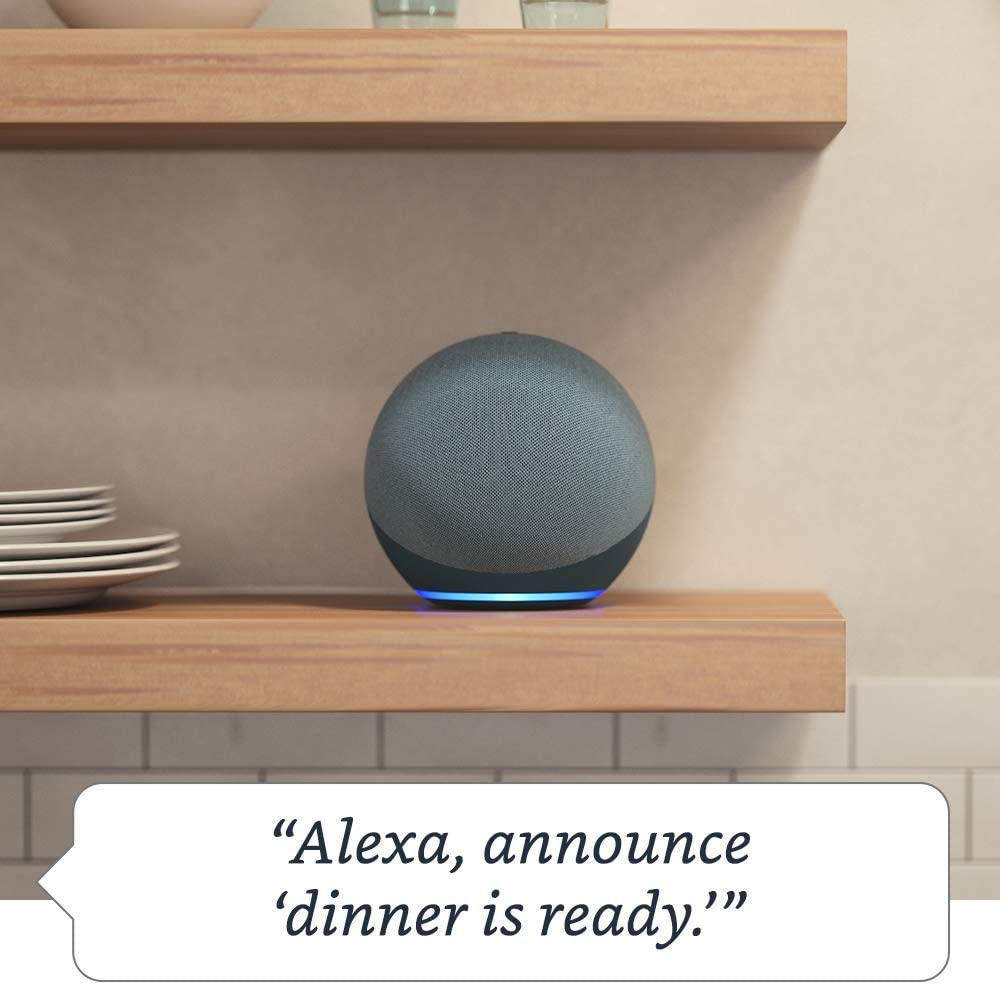
\includegraphics[width=0.4\textwidth]{./images/echodot4.jpg} % <- formatos PNG, JPG e PDF
	\caption[Amazon Echo 4th Generation smart speaker promotional material]{Amazon Echo 4th Gen Smart Speaker promotional material}
	\fonte{Amazon}
	\label{fig:dummy}
\end{figure}

\begin{quote}
    \textit{This device is a gem! When I’m busy in the kitchen, for example, and can’t get
    to a computer to find info or music to play, Alexa would be there to listen
    and do what I ask.} \\
    Customer review from \cite{GaoPanWangChen2018}
\end{quote}

Alongside the devices themselves, entirely new markets have emerged such as the third-party software extensions
called \textit{Alexa Skills} \cite{Alexa2022}.

These skills function much like mobile phone apps, extending and enhancing the functionality of the device, and
can be sold to users.

Developers are can then leverage the highly advanced machine learning models - which can be notoriously expensive to develop 
and maintain \cite{Phdata2021} - through \sigla{APIs}{Application Programming Interfaces} and focus exclusively on their application logic.

\begin{figure}[htb!]
	\centering
	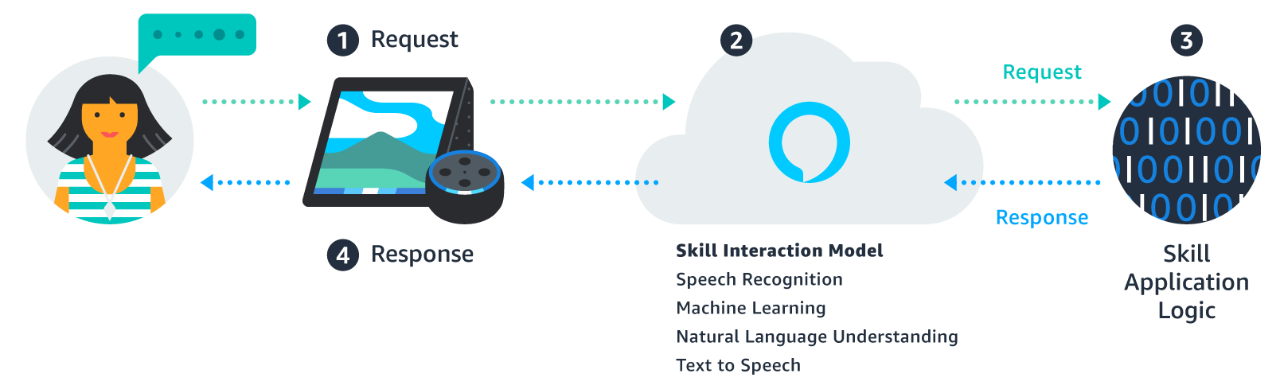
\includegraphics[width=0.9\textwidth]{./images/skills.png} % <- formatos PNG, JPG e PDF
	\caption[]{Diagram showing the steps of an interaction with an Alexa Skill}
    \fonte{\cite{Alexa2022}}
	\label{fig:dummy}
\end{figure}

More impressively, such technological advancements have been able to reach a considerable amount of households in
a short period in developed countries like the United States, a display of the power of the economy of scale and how
an extensible ecosystem can boost sales.

\begin{figure}[H]
	\centering
	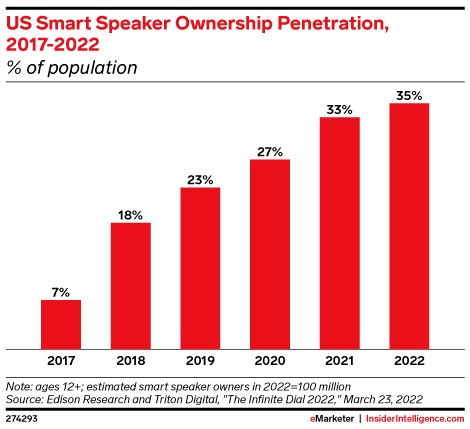
\includegraphics[width=0.6\textwidth]{./images/smartspeaker.png} % <- formatos PNG, JPG e PDF
	\caption[US Smart Speaker Penetration from 2017 to 2022]{US Smart Speaker Penetration from 2017 to 2022}
    \fonte{\cite{InsiderIntelligence2022}}
	\label{fig:dummy}
\end{figure}

On developing countries, such as Brazil, these innovations tend to have delayed
arrivals due to historical economic barriers but the potential customer base
has attracted big tech companies and their economic power, shortening the
delay.

\begin{figure}[h!]
	\centering
	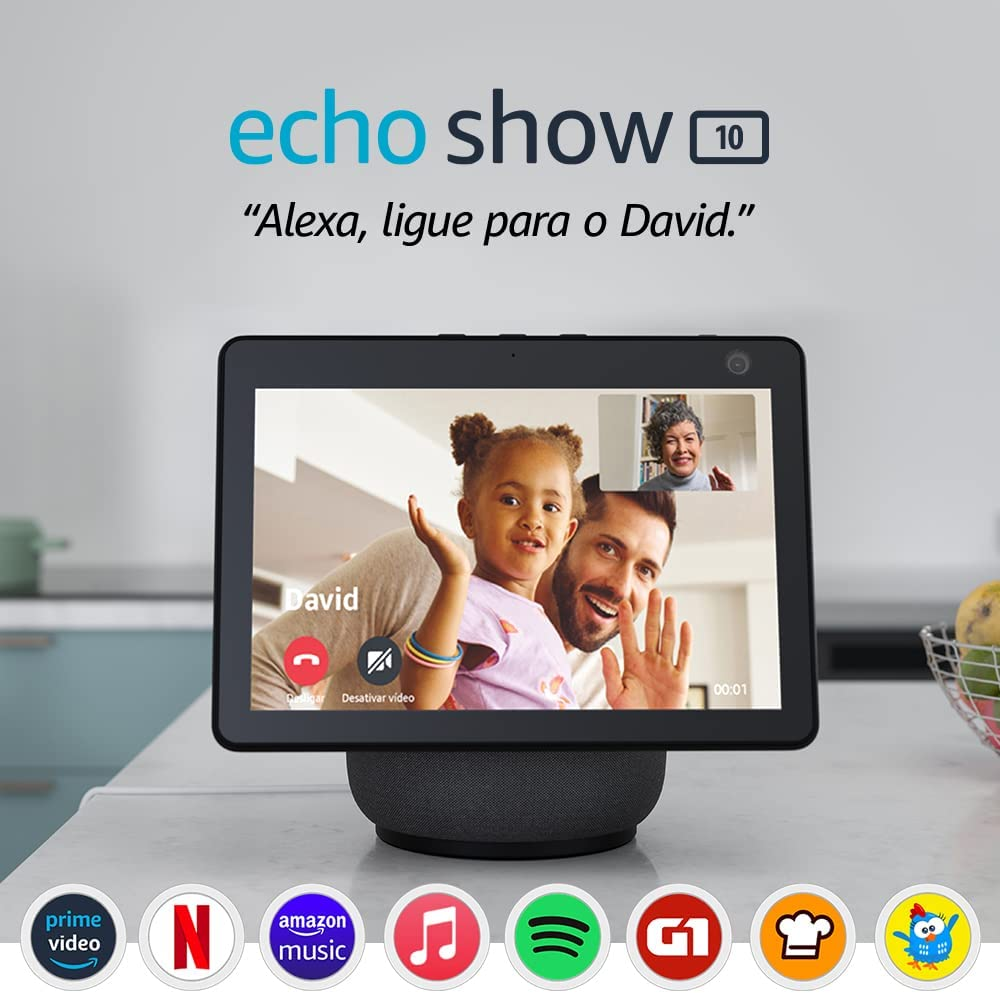
\includegraphics[width=0.4\textwidth]{./images/alexabr.jpg} % <- formatos PNG, JPG e PDF
	\caption[]{Localized promotional material for the Echo Show 10 targeting Brazilian customers}
    \fonte{Amazon}
	\label{fig:dummy}
\end{figure}

According to the research company IDC Brasil, the home automation market - in
which smart speakers are included - would have reached US\$ 298 million on
2021.

Although these advancements might seem entirely beneficial at first, countless
challenges have been found regarding privacy and ethical handling of personal
customer data \cite{Echoes2022} and overall negative experiences \cite{He2019}

These discussions are of the utter most importance given our current scenario
and have been brought up by recent literature but will be out of the scope of
our work.

\section{Motivation}

Even with all of these innovations that are impacting customer behaviors, one aspect of the stands out as not having changed 
significantly in the last couple of years: \textbf{Grocery Shopping}.

No ano passado, o setor alcançou um faturamento de R\$ 611,2 bilhões, por meio
da operação de todos os seus formatos e canais de distribuição (mercado de
vizinhança, supermercado, hipermercado, atacarejo e e-commerce). Com isso, o
resultado consolidado pelos supermercados representa 7,03\% do Produto Interno
Bruto (PIB) nacional.
https://www.abras.com.br/economia-e-pesquisa/ranking-abras/dados-gerais

https://www.abras.com.br/clipping/tecnologia/110172/a-evolucao-do-e-commerce-na-nova-era-pos-covid

Even after the COVID-19 pandemic, customer behavior has once again shifted back towards physical grocery shopping (add sources)

\section{Current scenario}

\subsection{Amazon Fresh}

\subsection{Caper.ai}

\subsection{Nextop}

\begin{figure}[!htb]
	\centering
	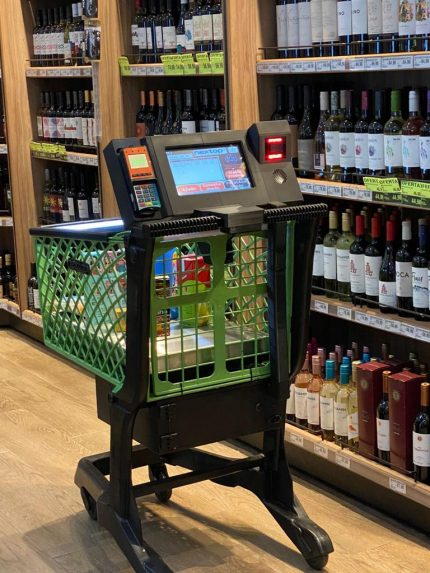
\includegraphics[width=0.4\textwidth]{./images/nextop.jpeg}
	\caption[]{Smart Cart® deployed to Brazilian supermarket}
    \fonte{Nextop}
	\label{fig:dummy}
\end{figure}


\section{Expected outcomes}

Develop a prototype of a smart shopping cart, with object recognition and
user interface.

\begin{itemize}
	\item Develop
	\item Desonerar autores da tediosa tarefa de formatar documentos academicos, permitindo sua concentracao no conteudo do mesmo.
	\item Understand the practical challenges of developing a deep-learning based product
\end{itemize}

\chapter{Theoretical Background}

In this section, we'll define in greater detail some of the relevant techniques
that were used in developing our prototype.

This section can be skipped for readers with domain familiarity.

\section{Deep Learning}

\section{Neural Networks}

\section{Strain Gauge}

\section{Load Cell}

\section{HX711}

\section{API}

\section{HTTP}

\section{JSON}

\section{SQL}

\section{SQLite}

%---------- Segundo Capitulo ----------
\chapter{Development}
\label{chap:desenv}

A seguir ilustra-se a forma de incluir figuras, tabelas, equac\~oes, siglas e simbolos no documento, obtendo indexacao automatica em suas respectivas listas. A numeracao sequencial de figuras, tabelas e equac\~oes ocorre de modo automatico. Referencias cruzadas sao obtidas atraves dos comandos {\ttfamily \textbackslash label\{\}} e {\ttfamily \textbackslash ref\{\}}. Por exemplo, nao e necessario saber que o numero deste capitulo e~\ref{chap:desenv} para colocar o seu numero no texto. Isto facilita muito a insercao, remocao ou relocacao de elementos numerados no texto (fato corriqueiro na escrita e correcao de um documento academico) sem a necessidade de renumera-los todos.

\section{Figuras}

Na figura~\ref{fig:dummy} e apresentado um exemplo de grafico flutuante. Esta figura aparece automaticamente na lista de figuras. Para uso avancado de graficos no \LaTeX, recomenda-se a consulta de literatura especializada~\cite{Goossens2007}.


\begin{figure}[!htb]
	\centering
	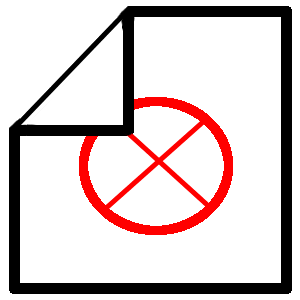
\includegraphics[width=0.2\textwidth]{./dummy.png} % <- formatos PNG, JPG e PDF
	\caption[Figure example]{Exemplo de uma figura onde aparece uma imagem sem nenhum significado especial.}
	\fonte{\cite{abnTeX2009}}
	\label{fig:dummy}
\end{figure}


\section{Tabelas}

Tambem e apresentado o exemplo da tabela~\ref{tab:correlacao}, que aparece automaticamente na lista de tabelas. Informac\~oes sobre a construcao de tabelas no \LaTeX\ podem ser encontradas na literatura especializada~\cite{Lamport1986,Buerger1989,Kopka2003,Mittelbach2004}.

\begin{table}[!htb]
	\centering
	\caption[Table example]{Exemplo de uma tabela mostrando a correlacao entre x e y.}
	\label{tab:correlacao}
	\begin{tabular}{cc}
		\hline 
		x & y \\
		\hline
		1 & 2 \\
		3 & 4 \\
		5 & 6 \\
		7 & 8 \\
		\hline 
	\end{tabular}
	\fonte{Autoria propria.}
\end{table}

\section{Equações}

A transformada de Laplace e dada na equacao~(\ref{eq:laplace}), enquanto a equacao~(\ref{eq:dft}) apresenta a formulacao da transformada discreta de Fourier bidimensional\footnote{Deve-se reparar na formatacao esteticamente perfeita destas equac\~oes!}.

\begin{equation}
X(s) = \int\limits_{t = -\infty}^{\infty} x(t) \, \text{e}^{-st} \, dt
\label{eq:laplace}
\end{equation}

\begin{equation}
F(u, v) = \sum_{m = 0}^{M - 1} \sum_{n = 0}^{N - 1} f(m, n) \exp \left[ -j 2 \pi \left( \frac{u m}{M} + \frac{v n}{N} \right) \right]
\label{eq:dft}
\end{equation}

\section{Siglas e símbolos}

O pacote \textsc{abn}\TeX\ permite ainda a definicao de siglas e simbolos com indexacao automatica atraves dos comandos {\ttfamily \textbackslash sigla\{\}\{\}} e {\ttfamily \textbackslash simbolo\{\}\{\}}. Por exemplo, o significado das siglas\sigla{CPGEI}{Programa de Pos-graduacao em Engenharia Eletrica e Informatica Industrial},\sigla{DAELN}{Departamento Academico de Eletronica} e\sigla{UTFPR}{Universidade Tecnologica Federal do Parana} aparecem automaticamente na lista de siglas, bem como o significado dos simbolos\simbolo{$\lambda$}{comprimento de onda},\simbolo{$v$}{velocidade} e\simbolo{$f$}{frequencia} aparecem automaticamente na lista de simbolos. Mais detalhes sobre o uso destes e outros comandos do \textsc{abn}\TeX\ sao encontrados na sua documentacao especifica~\cite{abnTeX2009}.


%---------- Terceiro Capitulo ----------
\chapter{Conclusions}

Espera-se que o uso do estilo de formatacao \LaTeX\ adequado as Normas para Elaboracao de Trabalhos Academicos da UTFPR ({\ttfamily normas-utf-tex.cls}) facilite a escrita de documentos no ambito desta instituicao e aumente a produtividade de seus autores. Para usuarios iniciantes em \LaTeX, alem da bibliografia especializada ja citada, existe ainda uma serie de recursos~\cite{CTAN2009} e fontes de informacao~\cite{TeX-Br2009,Wikibooks2009} disponiveis na Internet.

Recomenda-se o editor de textos Kile como ferramenta de composicao de documentos em \LaTeX\ para usuarios Linux. Para usuarios Windows recomenda-se o editor \TeX nicCenter~\cite{TeXnicCenter2009}. O \LaTeX\ normalmente ja faz parte da maioria das distribuic\~oes Linux, mas no sistema operacional Windows e necessario instalar o software \textsc{MiK}\TeX~\cite{MiKTeX2009}.

Alem disso, recomenda-se o uso de um gerenciador de referencias como o JabRef~\cite{JabRef2009} ou Mendeley~\cite{Mendeley2009} para a catalogacao bibliografica em um arquivo \textsc{Bib}\TeX, de forma a facilitar citac\~oes atraves do comando {\ttfamily \textbackslash cite\{\}} e outros comandos correlatos do pacote \textsc{abn}\TeX. A lista de referencias deste documento foi gerada automaticamente pelo software \LaTeX\ + \textsc{Bib}\TeX\ a partir do arquivo {\ttfamily reflatex.bib}, que por sua vez foi composto com o gerenciador de referencias JabRef.

O estilo de formatacao \LaTeX\ da UTFPR e este exemplo de utilizacao foram elaborados por Diogo Rosa Kuiaski (diogo.kuiaski@gmail.com) e Hugo Vieira Neto (hvieir@utfpr.edu.br), com contribuic\~oes de Cesar Vargas Benitez. Sugest\~oes de melhorias sao bem-vindas.


%---------- Referencias ----------
\clearpage % this is need for add +1 to pageref of bibstart used in 'ficha catalografica'.
\label{bibstart}
\bibliography{reflatex} % geracao automatica das referencias a partir do arquivo reflatex.bib
\label{bibend}

%---------- Apendices (opcionais) ----------
\apendice
\chapter{Nome do Apendice}

Use o comando {\ttfamily \textbackslash apendice} e depois comandos {\ttfamily \textbackslash chapter\{\}}
para gerar titulos de apendices.


% ---------- Anexos (opcionais) ----------
\anexo
\chapter{Nome do Anexo}

Use o comando {\ttfamily \textbackslash anexo} e depois comandos {\ttfamily \textbackslash chapter\{\}}
para gerar titulos de anexos.


% --------- Ordenacao Afabetica da Lista de siglas --------
%\textbf{* Observac\~oes:} a ordenacao alfabetica da lista de siglas ainda nao eh realizada de forma automatica, porem
% eh possivel se de realizar isto manualmente. Duas formas:
%
% ** Primeira forma)
%    A ordenacao eh feita com o auxilio do comando 'sort', disponivel em qualquer
% sistema Linux e UNIX, e tambem em sistemas Windows se instalado o coreutils (http://gnuwin32.sourceforge.net/packages/coreutils.htm)
% comandos para compilar e ordenar, supondo que seu arquivo se chame 'dissertacao.tex':
%
%      $ latex dissertacao
%      $ bibtex dissertacao && latex dissertacao
%      $ latex dissertacao
%      $ sort dissertacao.lsg > dissertacao.lsg.tmp
%      $ mv dissertacao.lsg.tmp dissertacao.lsg
%      $ latex dissertacao
%      $ dvipdf dissertacao.dvi
%
%
% ** Segunda forma)
%\textbf{Sugestao:} crie outro arquivo .tex para siglas e utilize o comando \sigla{sigla}{descricao}.
%Para incluir este arquivo no final do arquivo, utilize o comando \input{arquivo.tex}.
%Assim, Todas as siglas serao geradas na ultima pagina. Entao, devera excluir a ultima pagina da versao final do arquivo
% PDF do seu documento.


%-------- Citacoes ---------
% - Utilize o comando \citeonline{...} para citacoes com o seguinte formato: Autor et al. (2011).
% Este tipo de formato eh utilizado no comeco do paragrafo. P.ex.: \citeonline{autor2011}

% - Utilize o comando \cite{...} para citacoeses no meio ou final do paragrafo. P.ex.: \cite{autor2011}



%-------- Titulos com nomes cientificos (titulo, capitulos e secoes) ----------
% Regra para escrita de nomes cientificos:
% Os nomes devem ser escritos em italico, 
%a primeira letra do primeiro nome deve ser em maiusculo e o restante em minusculo (inclusive a primeira letra do segundo nome).
% VEJA os exemplos abaixo.
% 
% 1) voce nao quer que a secao fique com uppercase (caixa alta) automaticamente:
%\section[nouppercase]{\MakeUppercase{Estudo dos efeitos da radiacao ultravioleta C e TFD em celulas de} {\textit{Saccharomyces boulardii}}
%
% 2) por padrao os cases (maiusculas/minuscula) sao ajustados automaticamente, voce nao precisa usar makeuppercase e afins.
% \section{Introducao} % a introducao sera posta no texto como INTRODUCAO, automaticamente, como a norma indica.


\end{document}
